

\documentclass{article}
\usepackage{graphicx}
\usepackage{amsmath}
\usepackage{amssymb}
\usepackage{listings}
\usepackage[margin=1in]{geometry}
\usepackage{xcolor}
\usepackage{tikz}
\usetikzlibrary{shapes, arrows, positioning, calc}
\usepackage{tcolorbox}
% Define colors for syntax highlighting
\definecolor{codegreen}{rgb}{0,0.6,0}
\definecolor{codegray}{rgb}{0.5,0.5,0.5}
\definecolor{codepurple}{rgb}{0.58,0,0.82}
\definecolor{backcolour}{rgb}{0.95,0.95,0.92}

% Python style for highlighting
\lstdefinestyle{pythonstyle}{
    backgroundcolor=\color{backcolour},   
    commentstyle=\color{codegreen},
    keywordstyle=\color{magenta},
    numberstyle=\tiny\color{codegray},
    stringstyle=\color{codepurple},
    basicstyle=\ttfamily\footnotesize,
    breakatwhitespace=false,         
    breaklines=true,                 
    captionpos=b,                    
    keepspaces=true,                 
    numbers=left,                    
    numbersep=5pt,                  
    showspaces=false,                
    showstringspaces=false,
    showtabs=false,                  
    tabsize=2
}
\lstset{style=pythonstyle}

\title{Backpropagation: A Simple Derivation and Implementation}
\author{Deep Learning Class}
\date{\today}

\begin{document}
\maketitle

\section{Recap: SGD to Minimize the Loss Function}

We use Stochastic Gradient Descent (SGD) to minimize the loss function $L(w)$:
\begin{equation}
    w_{\text{new}} = w_{\text{old}} - \eta \cdot \nabla L
\end{equation}
where $\eta$ is the learning rate (e.g., $\eta = 0.01$).

The gradient $\nabla L$ tells us the direction of fastest \textbf{increase} of the loss function. Therefore, moving in the negative gradient direction $-\nabla L$ gives us the direction of fastest \textbf{decrease}.

To use SGD, we need to compute the gradient:
\begin{equation}
    \nabla L = \begin{bmatrix}
        \frac{\partial L}{\partial w^{(1)}} \\
        \vdots \\
        \frac{\partial L}{\partial w^{(n)}}
    \end{bmatrix}
\end{equation}
where $\frac{\partial L}{\partial w^{(i)}}$ calculates how sensitive is $L$ to changing $w_i$.

\paragraph{The key challenge:} How do we efficiently compute $\frac{\partial L}{\partial w}$ for each weight in a network with potentially millions of parameters? 



\textbf{Key insight:} Computing this naively would be computationally infeasible. Backpropagation solves this efficiently using the chain rule.

\section{Recall Chain Rule}

Let's start with a simple example to build intuition. Consider a single neuron with:
- Input: $a^{(L-1)}$ (activation from previous layer)
- Weight: $w^{(L)}$
- Bias: $b^{(L)}$
- Output: $a^{(L)}$

\begin{center}
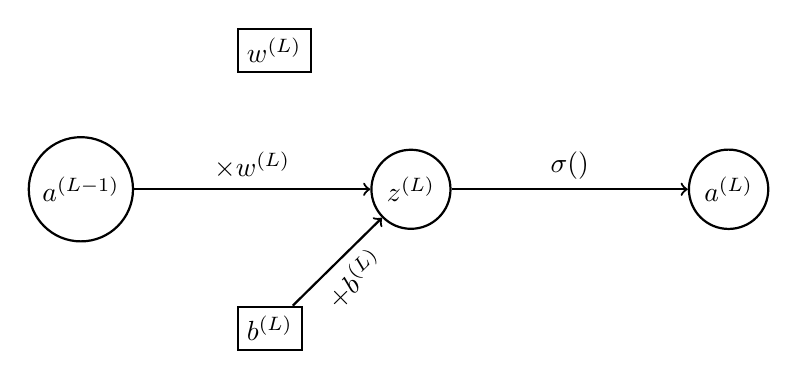
\begin{tikzpicture}[
    node distance=2cm,
    neuron/.style={circle, draw, thick, minimum size=1cm},
    weight/.style={rectangle, draw, thick, minimum size=0.5cm}
]
    % Nodes
    \node[neuron] (input) {$a^{(L-1)}$};
    \node[weight] (weight) [above right=1cm and 1.5cm of input] {$w^{(L)}$};
    \node[weight] (bias) [below right=1cm and 1.5cm of input] {$b^{(L)}$};
    \node[neuron] (output) [right=3cm of input] {$z^{(L)}$};
    \node[neuron] (output2) [right=3cm of output] {$a^{(L)}$};
    % Connections
    \draw[->, thick] (input) -- node[above, sloped] {$\times w^{(L)}$} (output);
    \draw[->, thick] (bias) -- node[below, sloped] {$+b^{(L)}$} (output);
    \draw[->, thick] (output) -- node[above, sloped] {$\sigma()$} (output2);
\end{tikzpicture}
\end{center}

The forward computation is:
\begin{equation}
    z^{(L)} = a^{(L-1)} \cdot w^{(L)} + b^{(L)}
\end{equation}
\begin{equation}
    a^{(L)} = \sigma(z^{(L)})
\end{equation}

where $\sigma$ is the activation function.


% ------% ------% ------
\begin{tcolorbox}[
    colback=blue!5!white,
    colframe=blue!50!black,
    title={\textbf{Melting bias into the weights}},
    fonttitle=\bfseries,
    sharp corners,
    boxrule=1pt,
    left=6pt,
    right=6pt,
    top=6pt,
    bottom=6pt
]
\footnotesize
In practice, we can simplify our notation by incorporating the bias into the weight matrix. We add a fixed neuron with value 1 to each layer:

\begin{equation}
    z = \begin{bmatrix} w_1 & w_2 & \cdots & w_n & b \end{bmatrix} \begin{bmatrix} a_1 \\ a_2 \\ \vdots \\ a_n \\ 1 \end{bmatrix} = \tilde{W} \tilde{a}
\end{equation}

This allows us to treat bias as just another weight connected to a neuron that always outputs 1.

\begin{center}
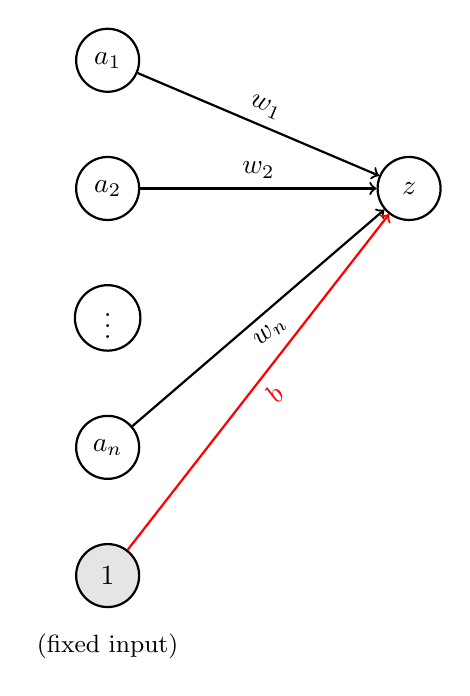
\begin{tikzpicture}[
    node distance=1.5cm,
    neuron/.style={circle, draw, thick, minimum size=0.8cm},
    bias/.style={circle, draw, thick, minimum size=0.8cm, fill=gray!20}
]
    % Input neurons
    \node[neuron] (a1) {$a_1$};
    \node[neuron] (a2) [below=0.8cm of a1] {$a_2$};
    \node[neuron] (dots) [below=0.8cm of a2] {$\vdots$};
    \node[neuron] (an) [below=0.8cm of dots] {$a_n$};
    \node[bias] (bias) [below=0.8cm of an] {$1$};
    
    % Output neuron
    \node[neuron] (output) [right=3cm of a2] {$z$};
    
    % Connections
    \draw[->, thick] (a1) -- node[above, sloped] {$w_1$} (output);
    \draw[->, thick] (a2) -- node[above, sloped] {$w_2$} (output);
    \draw[->, thick] (an) -- node[below, sloped] {$w_n$} (output);
    \draw[->, thick, red] (bias) -- node[below, sloped] {$b$} (output);
    
    % Label
    \node[below=0.2cm of bias] {\small (fixed input)};
\end{tikzpicture}
\end{center}
\end{tcolorbox}
% ------% ------% ------

\subsection{Computing Gradients Using the Chain Rule}

To find how the loss $L$ changes with respect to the weight $w^{(L)}$, we use the chain rule:

\begin{equation}
    \frac{\partial L}{\partial w^{(L)}} = \frac{\partial L}{\partial a^{(L)}} \cdot \frac{\partial a^{(L)}}{\partial z^{(L)}} \cdot \frac{\partial z^{(L)}}{\partial w^{(L)}}
\end{equation}

Let's compute each term:
- $\frac{\partial z^{(L)}}{\partial w^{(L)}} = a^{(L-1)}$ (from the forward equation)
- $\frac{\partial a^{(L)}}{\partial z^{(L)}} = \sigma'(z^{(L)})$ (derivative of activation function)
- $\frac{\partial L}{\partial a^{(L)}}$ depends on what comes after this layer

This gives us:
\begin{equation}
    \frac{\partial L}{\partial w^{(L)}} = a^{(L-1)} \cdot \sigma'(z^{(L)}) \cdot \frac{\partial L}{\partial a^{(L)}}
\end{equation}





\section{The Backpropagation Algorithm: A Game of Blame}

Backpropagation is the algorithm that allows us to train deep neural networks by efficiently computing the gradient of the loss function with respect to every weight and bias in the network. The core challenge is untangling the complex web of interconnected calculations to see how a single weight in an early layer affects the final output error.

The key insight of backpropagation is to frame this as a ``game of blame." We start at the end, where the error is obvious, and propagate a ``blame signal" backwards through the network, layer by layer. This signal tells us how much each component contributed to the final error.

\subsection{Defining the Blame Signal: The Delta Term}

To formalize this, we introduce a crucial intermediate quantity, $\delta^{(l)}$, which we can think of as the \textbf{blame signal} for layer $l$. It is defined as the partial derivative of the loss function $L$ with respect to the pre-activation value $z^{(l)}$ of that layer:

\begin{equation}
    \delta^{(l)} := \frac{\partial L}{\partial z^{(l)}}
\end{equation}

By defining our blame signal this way, we are essentially asking: ``How much did the pre-activation value of each neuron in layer $l$ contribute to the final loss?" This turns out to be the perfect quantity to track as we move backward through the network.

\subsection{The Four Fundamental Equations of Blame}

\textbf{1. Starting the Game: Blame at the Output Layer}

We begin by calculating the blame for the very last layer, $L$. This is the most direct step, as the output layer is closest to the loss function. Using the chain rule, we connect the final loss to the pre-activation $z^{(L)}$:

\begin{align}
    \delta^{(L)} &= \frac{\partial L}{\partial z^{(L)}} \\
    &= \frac{\partial L}{\partial a^{(L)}} \frac{\partial a^{(L)}}{\partial z^{(L)}} \nonumber \\
    &= \frac{\partial L}{\partial a^{(L)}} \odot \sigma'(z^{(L)}) \label{eq:bp1}
\end{align}
This first equation calculates the initial blame. For a simple squared error loss, $\frac{\partial L}{\partial a^{(L)}}$ is just $(a^{(L)} - y)$, which is literally the error in the network's prediction. So, $\delta^{(L)}$ is the final prediction error, scaled by how sensitive the activation function was to its input.

\textbf{2. Propagating the Blame Backwards}

This is the heart of backpropagation. Once we know the blame at layer $l+1$, how do we determine the blame for the preceding layer $l$? The blame must flow backward through the weights that connected them. This gives us the recursive relationship:

\begin{equation}
    \delta^{(l)} = \left( (W^{(l+1)})^T \delta^{(l+1)} \right) \odot \sigma'(z^{(l)}) \label{eq:bp2}
\end{equation}
This equation elegantly states that the blame at layer $l$ is the blame from the next layer ($\delta^{(l+1)}$) propagated backward through the transpose of the weight matrix $W^{(l+1)}$, and then scaled by the local gradient of the activation function at layer $l$. This allows us to move backward through the network, from $\delta^{(L)}$ to $\delta^{(L-1)}$, and so on.

\textbf{3. Using Blame to Correct Weights}

Calculating the blame signal is only useful if we can use it to make corrections. The gradient for the weights of any layer $l$ can be found directly using that layer's blame signal, $\delta^{(l)}$, and the activations from the previous layer, $a^{(l-1)}$:

\begin{equation}
    \frac{\partial L}{\partial W^{(l)}} = \delta^{(l)} (a^{(l-1)})^T \label{eq:bp3}
\end{equation}
This tells us how to adjust the weights. The update is proportional to the blame signal ($\delta^{(l)}$) and the signal that was flowing through the weights during the forward pass ($a^{(l-1)}$).

\textbf{4. Using Blame to Correct Biases}

Similarly, the gradient for the biases is even simpler. Since a bias is just added to the pre-activation value $z^{(l)}$, its influence on the loss is directly measured by the blame signal $\delta^{(l)}$:

\begin{equation}
    \frac{\partial L}{\partial b^{(l)}} = \delta^{(l)} \label{eq:bp4}
\end{equation}
This shows that the required change for a bias is simply equal to the blame assigned to its neuron.

By introducing $\delta$, we transform a tangled mess of derivatives into a clean, two-stage process: first, a backward pass to compute the blame signals for each layer (Equations \ref{eq:bp1} and \ref{eq:bp2}), followed by a step to calculate the desired weight and bias updates for each layer based on that blame (Equations \ref{eq:bp3} and \ref{eq:bp4}).



\subsection{The Power of Vectorization: From Neurons to Networks}

A key reason this formulation is so powerful is that the four fundamental equations are already written in their complete, vectorized form. We don't need a different set of rules for networks with more layers or neurons—the matrix and vector operations handle the complexity automatically.

Let's appreciate what this notation accomplishes:
\begin{itemize}
    \item \textbf{No Messy Summations:} Without vectorization, the ``blame propagation" equation (Equation \ref{eq:bp2}) for a single neuron $j$ in layer $l$ would be a complex sum over all $k$ neurons in layer $l+1$:
    $$ \delta_j^{(l)} = \left( \sum_{k=1}^{n^{(l+1)}} W_{kj}^{(l+1)} \delta_k^{(l+1)} \right) \sigma'(z_j^{(l)}) $$
    The vectorized form, $\left( (W^{(l+1)})^T \delta^{(l+1)} \right) \odot \sigma'(z^{(l)})$, computes this for all neurons in the layer in a single, clean operation. The matrix-vector product $(W^{(l+1)})^T \delta^{(l+1)}$ elegantly performs all the necessary summations.

    \item \textbf{The Outer Product for the Weight Gradient:} Equation \ref{eq:bp3} for the weight gradient, $\frac{\partial L}{\partial W^{(l)}} = \delta^{(l)} (a^{(l-1)})^T$, is a perfect example of this elegance. It uses an \textbf{outer product} to compute the entire gradient matrix in one step.
    
    Here's how it works: Let's say the previous layer $l-1$ has $n$ neurons and the current layer $l$ has $m$ neurons.
    \begin{itemize}
        \item The blame signal $\delta^{(l)}$ is a column vector of shape ($m \times 1$).
        \item The activation vector from the previous layer, $a^{(l-1)}$, is a column vector of shape ($n \times 1$). Its transpose, $(a^{(l-1)})^T$, is a row vector of shape ($1 \times n$).
    \end{itemize}
    
    Multiplying a column vector by a row vector yields a matrix:
    $$ \underset{(m \times 1)}{\delta^{(l)}} \underset{(1 \times n)}{(a^{(l-1)})^T} = 
       \begin{bmatrix} \delta_1^{(l)} \\ \delta_2^{(l)} \\ \vdots \\ \delta_m^{(l)} \end{bmatrix}
       \begin{bmatrix} a_1^{(l-1)} & a_2^{(l-1)} & \cdots & a_n^{(l-1)} \end{bmatrix}
       =
       \underset{(m \times n)}{\begin{bmatrix}
       \delta_1^{(l)} a_1^{(l-1)} & \delta_1^{(l)} a_2^{(l-1)} & \cdots & \delta_1^{(l)} a_n^{(l-1)} \\
       \delta_2^{(l)} a_1^{(l-1)} & \delta_2^{(l)} a_2^{(l-1)} & \cdots & \delta_2^{(l)} a_n^{(l-1)} \\
       \vdots & \vdots & \ddots & \vdots \\
       \delta_m^{(l)} a_1^{(l-1)} & \delta_m^{(l)} a_2^{(l-1)} & \cdots & \delta_m^{(l)} a_n^{(l-1)}
       \end{bmatrix}}
    $$
    The resulting $m \times n$ matrix has the exact same dimensions as the weight matrix $W^{(l)}$. Each element $(i,j)$ of this matrix correctly represents $\frac{\partial L}{\partial W_{ij}^{(l)}}$, which is the blame from neuron $i$ multiplied by the activation from neuron $j$ that fed into it.

    \item \textbf{Parallel Computation:} This formulation isn't just for cleaner notation; it maps directly to how modern hardware (like GPUs) performs computations. Matrix multiplications are highly parallelizable, making the backpropagation algorithm incredibly efficient on a large scale.
\end{itemize}

This elegance is the beauty of backpropagation. The same four equations describe the learning process for a simple network with a handful of neurons and a massive foundation model with billions of them. The logic of propagating ``blame" remains identical; only the size of the matrices changes.




% ------% ------% ------
\begin{tcolorbox}[
    colback=blue!5!white,
    colframe=blue!50!black,
    title={\textbf{sensitivity of the activation function}},
    fonttitle=\bfseries,
    sharp corners,
    boxrule=1pt,
    left=6pt,
    right=6pt,
    top=6pt,
    bottom=6pt
]
% \footnotesize
During backpropagation, the derivative of the activation function, $\sigma'(z^{(l)})$, acts as a \textbf{gate} that controls how much gradient is allowed to flow backward through each neuron. The value of this derivative determines if the gate is open, closed, or somewhere in between. This gating mechanism is critical for understanding why some activation functions are preferred over others in deep networks.\\

\textbf{The Sigmoid Bottleneck:}
The sigmoid activation function squashes any real-valued input into the range (0, 1). It's defined as:
\begin{equation}
    \sigma(z) = \frac{1}{1 + e^{-z}}
\end{equation}
The derivative of the sigmoid function is given by:
\begin{equation}
    \sigma'(z) = \sigma(z)(1 - \sigma(z))
\end{equation}
\begin{itemize}
    \item \textbf{The Gate's Problem:} The maximum value of this derivative is only \textbf{0.25} (when $z=0$). For inputs far from zero (large positive or negative $z$), the neuron becomes saturated, and the derivative $\sigma'(z)$ approaches 0.
    \item \textbf{The Consequence:} This means the sigmoid gate is, at best, only partially open and is often nearly closed. In a deep network, these small derivative values are multiplied together at each layer. This causes the gradient to shrink exponentially as it flows backward, a famous problem known as \textbf{vanishing gradients}. The signal becomes too weak to update the early layers of the network effectively.
\end{itemize}

\textbf{The ReLU Superhighway}

The derivative of the Rectified Linear Unit (ReLU), $\text{ReLU}(z) = \max(0, z)$, is a simple step function:
\begin{equation}
    \text{ReLU}'(z) = \begin{cases}
        1 & \text{if } z > 0 \\
        0 & \text{if } z \leq 0
    \end{cases}
\end{equation}
\begin{itemize}
    \item \textbf{The Gate's Behavior:} The ReLU gate is elegantly simple: it's either \textbf{fully open} (value 1) or \textbf{fully closed} (value 0).
    \item \textbf{The Consequence:} If a neuron was active during the forward pass ($z>0$), the gradient passes through it unchanged during backpropagation (multiplied by 1). This allows the error signal to travel back through many layers without diminishing, acting like a gradient superhighway. This reliable gradient flow is a primary reason why \textbf{ReLU and its variants are the default choice} for most deep neural networks.
\end{itemize}

\end{tcolorbox}
% ------% ------% ------


\section{Key Takeaways}

\begin{enumerate}
    \item \textbf{Backpropagation = Chain Rule + Smart Bookkeeping}: Just careful application of calculus.
    
    \item The algorithm always works in two distinct passes:
    \begin{itemize}
        \item \textbf{Forward pass:} Starting with the input, compute the activations for each layer sequentially and store these intermediate values (activations $a^{(l)}$ and pre-activations $z^{(l)}$).
        \item \textbf{Backward pass:} Starting from the final loss, compute the gradients by propagating the error signal $\delta^{(l)}$ backwards, from the last layer to the first.
    \end{itemize}
    \item \textbf{Memory Trade-off}: We must store intermediate values from the forward pass, which is why training requires more memory than inference.
    
    \item \textbf{Computational Efficiency}: By traversing the graph once forward and once backward, we compute all gradients in $O(n)$ time ($n$ is total number of parameters).
    
    \item The error signal $\delta^{(l)} = \frac{\partial L}{\partial z^{(l)}}$ is the central quantity, as it neatly encapsulates how much each neuron in layer $l$ is responsible for the overall loss.
    
    \item Modern deep learning frameworks like PyTorch and TensorFlow have automated this process with \textbf{automatic differentiation} (autodiff). Autodiff generalizes backpropagation, allowing it to compute gradients for any arbitrary computational graph, not just layered neural networks. But understanding the principles helps in:
    \begin{itemize}
        \item Debugging gradient issues
        \item Designing custom layers
        \item Understanding memory requirements
        \item Optimizing performance
    \end{itemize}
\end{enumerate}










\section{Simple Implementation in Python}

Let's implement a simple example to demonstrate backpropagation for a 2-layer network.\\
\textbf{Note:} In this implementation, we handle bias separately for clarity. In practice, you can use the bias trick by appending a column of 1's to your input data and incorporating bias into the weight matrix.\\
\begin{lstlisting}[language=Python, caption=Simple Backpropagation Implementation]
import numpy as np
# https://colab.research.google.com/drive/1-ax4mCREZVvse9-zNv6pyuQdyCeA4nXA
# --- Activation Functions and Their Derivatives ---

def relu(z):
    """
    Rectified Linear Unit (ReLU) activation function.
    Returns z if z > 0, otherwise returns 0.
    """
    return np.maximum(0, z)

def relu_derivative(z):
    """
    Derivative of the ReLU function.
    
    Note on non-differentiability at z=0:
    Mathematically, the derivative of ReLU is undefined at z=0. However, in practice,
    this is not an issue. We can simply assign the derivative to be 0 or 1 at that
    point. The chance of a floating-point number being exactly zero is extremely
    small, so this choice has no significant impact on the training process.
    Here, we define it as 0.
    """
    return (z > 0).astype(float)

def sigmoid(z):
    """
    Sigmoid activation function. Used for the output layer for binary
    classification to squash the output between 0 and 1.
    """
    # Clip z to avoid overflow in exp for very large negative numbers
    z = np.clip(z, -500, 500)
    return 1 / (1 + np.exp(-z))

def sigmoid_derivative(z):
    """Derivative of the sigmoid function."""
    s = sigmoid(z)
    return s * (1 - s)

# --- Network Architecture ---

def initialize_parameters(n_input, n_hidden, n_output):
    """
    Initializes weights and biases for a 2-layer network.
    """
    np.random.seed(42) # for reproducibility
    W1 = np.random.randn(n_input, n_hidden) * 0.1
    b1 = np.zeros((1, n_hidden))
    W2 = np.random.randn(n_hidden, n_output) * 0.1
    b2 = np.zeros((1, n_output))
    
    parameters = {"W1": W1, "b1": b1, "W2": W2, "b2": b2}
    return parameters

def forward_pass(X, parameters):
    """
    Performs a forward pass through the network.
    
    Architecture: Input -> Linear -> ReLU -> Linear -> Sigmoid -> Output
    """
    # Retrieve parameters
    W1, b1, W2, b2 = parameters["W1"], parameters["b1"], parameters["W2"], parameters["b2"]
    
    # Layer 1 (Hidden)
    z1 = np.dot(X, W1) + b1
    a1 = relu(z1)
    
    # Layer 2 (Output)
    z2 = np.dot(a1, W2) + b2
    a2 = sigmoid(z2)
    
    # Store intermediate values in a cache for use in backpropagation
    cache = {"z1": z1, "a1": a1, "z2": z2, "a2": a2}
    return a2, cache

def compute_loss(y_pred, y_true):
    """
    Computes the Mean Squared Error loss.
    """
    m = y_true.shape[0] # number of samples
    loss = (1 / (2 * m)) * np.sum((y_pred - y_true)**2)
    return loss

def backward_pass(X, y_true, parameters, cache):
    """
    Performs the backward pass (backpropagation) to compute gradients.
    """
    m = X.shape[0]
    
    # Retrieve parameters and cached values
    W1, W2 = parameters["W1"], parameters["W2"]
    a1, a2, z1, z2 = cache["a1"], cache["a2"], cache["z1"], cache["z2"]
    
    # --- Step 1: Compute error at the Output Layer ---
    # This is delta2 in our equations, the "blame" for the final layer.
    # It's the derivative of the loss w.r.t z2.
    # dL/dz2 = dL/da2 * da2/dz2
    dL_da2 = (a2 - y_true) / m            # Derivative of MSE loss w.r.t a2
    delta2 = dL_da2 * sigmoid_derivative(z2) # Element-wise product
    
    # --- Step 2: Compute gradients for the Output Layer parameters (W2, b2) ---
    dW2 = np.dot(a1.T, delta2)
    db2 = np.sum(delta2, axis=0, keepdims=True)
    
    # --- Step 3: Propagate the error to the Hidden Layer ---
    # This is delta1, the "blame" for the hidden layer.
    # dL/dz1 = (dL/dz2 * dz2/da1) * da1/dz1
    delta1 = np.dot(delta2, W2.T) * relu_derivative(z1)
    
    # --- Step 4: Compute gradients for the Hidden Layer parameters (W1, b1) ---
    dW1 = np.dot(X.T, delta1)
    db1 = np.sum(delta1, axis=0, keepdims=True)
    
    grads = {"dW1": dW1, "db1": db1, "dW2": dW2, "db2": db2}
    return grads

def update_parameters(parameters, grads, learning_rate):
    """
    Updates parameters using gradient descent.
    """
    parameters["W1"] -= learning_rate * grads["dW1"]
    parameters["b1"] -= learning_rate * grads["db1"]
    parameters["W2"] -= learning_rate * grads["dW2"]
    parameters["b2"] -= learning_rate * grads["db2"]
    return parameters

# --- Main Execution ---
if __name__ == "__main__":
    # Create a simple dataset (XOR problem)
    X = np.array([[0, 0], [0, 1], [1, 0], [1, 1]])
    y = np.array([[0], [1], [1], [0]])
    
    # Network configuration
    n_input, n_hidden, n_output = 2, 10, 1
    
    # Initialize parameters
    parameters = initialize_parameters(n_input, n_hidden, n_output)
    
    # Training loop
    learning_rate = 1.0
    epochs = 1500
    
    for i in range(epochs):
        # 1. Forward pass
        y_pred, cache = forward_pass(X, parameters)
        
        # 2. Compute loss
        loss = compute_loss(y_pred, y)
        
        # 3. Backward pass
        grads = backward_pass(X, y, parameters, cache)
        
        # 4. Update parameters
        parameters = update_parameters(parameters, grads, learning_rate)
        
        # Print loss every 100 epochs
        if i % 100 == 0:
            print(f"Epoch {i}, Loss: {loss:.6f}")
            
    # Test the trained network
    print("\n--- Testing Trained Network ---")
    final_predictions, _ = forward_pass(X, parameters)
    
    # Round predictions to 0 or 1 for clarity
    binary_predictions = (final_predictions > 0.5).astype(int)
    
    print("Input (X):")
    print(X)
    print("\nTarget (y):")
    print(y)
    print("\nFinal Predictions (raw):")
    print(final_predictions)
    print("\nFinal Predictions (binary):")
    print(binary_predictions)
\end{lstlisting}








\section{Computational Graphs and Automatic Differentiation}

\subsection{Visualizing Computation as a Graph}

As shown in the textbook (Section 5.3.2), we can represent any computation as a directed graph where:
- Nodes represent variables or operations
- Edges represent dependencies

For our simple network:

\begin{center}
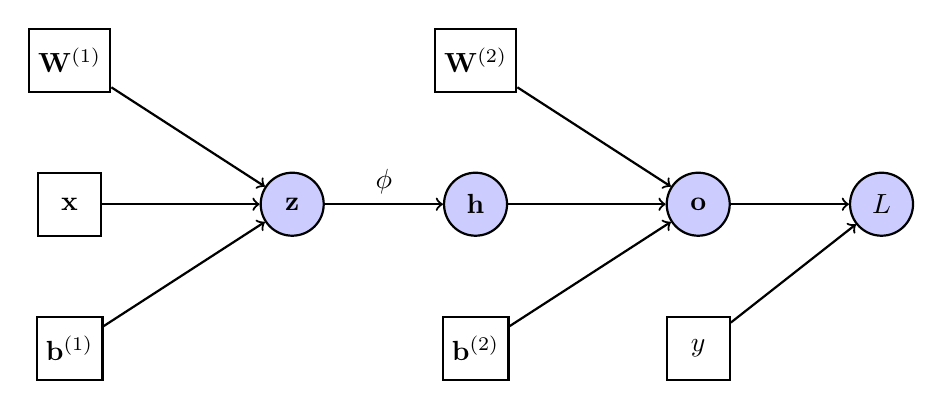
\begin{tikzpicture}[
node distance=2cm,
var_node/.style={rectangle, draw, thick, minimum size=0.8cm},
op_node/.style={circle, draw, thick, fill=blue!20, minimum size=0.8cm}
]
% Input layer
\node[var_node] (x) {$\mathbf{x}$};
\node[var_node] (W1) [above=1cm of x] {$\mathbf{W}^{(1)}$};
\node[var_node] (b1) [below=1cm of x] {$\mathbf{b}^{(1)}$};

% Hidden layer computation
\node[op_node] (z) [right=2cm of x] {$\mathbf{z}$};
\node[op_node] (h) [right=1.5cm of z] {$\mathbf{h}$};

% Output layer
\node[var_node] (W2) [above=1cm of h] {$\mathbf{W}^{(2)}$};
\node[var_node] (b2) [below=1cm of h] {$\mathbf{b}^{(2)}$};
\node[op_node] (o) [right=2cm of h] {$\mathbf{o}$};

% Loss
\node[var_node] (y) [below=1cm of o] {$y$};
\node[op_node] (L) [right=1.5cm of o] {$L$};

% Edges
\draw[->, thick] (x) -- (z);
\draw[->, thick] (W1) -- (z);
\draw[->, thick] (b1) -- (z);
\draw[->, thick] (z) -- (h) node[midway, above] {$\phi$};
\draw[->, thick] (h) -- (o);
\draw[->, thick] (W2) -- (o);
\draw[->, thick] (b2) -- (o);
\draw[->, thick] (o) -- (L);
\draw[->, thick] (y) -- (L);
\end{tikzpicture}
\end{center}




\newpage 



\section{Weight Initialization: Setting Up for Success}

In our simple implementation, we initialized weights using a small, arbitrary random scaling factor. While this prevents weights from being too large, it's a blunt instrument. 
For deep networks, the specific scale of initialization is often the deciding factor between a network that trains successfully and one that fails completely.

\subsection{The Core Problem: Unstable Signal Variance}

A neural network is fundamentally a pipeline of sequential computations. Signals—activations during the forward pass and gradients during the backward pass—travel through this pipeline. The variance of these signals can be thought of as their ``energy."

\begin{itemize}
    \item \textbf{Exploding Signal:} If the variance increases layer by layer, the signal can grow exponentially until it becomes enormous (NaNs). This leads to exploding gradients and a useless model.
    \item \textbf{Vanishing Signal:} If the variance decreases layer by layer, the signal can shrink exponentially until it becomes virtually zero. This leads to vanishing gradients, where the early layers of the network receive no learning signal and their weights are never updated.
\end{itemize}

The goal of a good initialization strategy is to ensure that, at the beginning of training, the variance of both the activations and the backpropagated gradients remains roughly constant as they pass through each layer.

\subsection{The Statistical Rationale: Fan-in and Fan-out}

Let's analyze the variance of a single neuron's pre-activation, $z = \sum_{i=1}^{n} w_i x_i$. To simplify, we make a few reasonable assumptions for the start of training:
\begin{itemize}
    \item The inputs $x_i$ and weights $w_i$ are independent and identically distributed.
    \item Both inputs and weights have a mean of 0.
    \item The input features are scaled to have a variance of 1, i.e., $\text{Var}(x) = 1$.
\end{itemize}

Using the properties of variance, the variance of $z$ is:
\begin{equation}
    \text{Var}(z) = \text{Var}\left(\sum_{i=1}^{n} w_i x_i\right) = \sum_{i=1}^{n} \text{Var}(w_i x_i)
\end{equation}
Since $w_i$ and $x_i$ are independent with zero mean, $\text{Var}(w_i x_i) = \text{Var}(w_i)\text{Var}(x_i)$. This gives us:
\begin{equation}
    \text{Var}(z) = n \cdot \text{Var}(w) \cdot \text{Var}(x)
\end{equation}
If we want the output variance to equal the input variance, i.e., $\text{Var}(z) = \text{Var}(x) = 1$, we must set the variance of the weights to:
\begin{equation}
    n \cdot \text{Var}(w) = 1 \implies \text{Var}(w) = \frac{1}{n}
\end{equation}
Here, $n$ is the number of inputs to the neuron, which is known as the \textbf{fan-in} ($n_{\text{in}}$) of the layer.

This logic ensures the forward pass is stable. However, for the backward pass, a similar analysis shows that to keep the gradient variance stable, we need $\text{Var}(w) = \frac{1}{n_{\text{out}}}$, where \textbf{fan-out} ($n_{\text{out}}$) is the number of neurons in the next layer.

\subsection{Xavier/Glorot Initialization (for Sigmoid \& Tanh)}

So which should we choose, fan-in or fan-out? The Xavier/Glorot initialization proposes a compromise: use the average of the two. It is designed for activations like sigmoid and tanh that are symmetric around zero.
\begin{equation}
    \text{Var}(W) = \frac{2}{n_{\text{in}} + n_{\text{out}}}
\end{equation}
To achieve this variance, we can sample weights from:
\begin{itemize}
    \item A normal distribution: $W \sim \mathcal{N}\left(0, \sqrt{\frac{2}{n_{\text{in}} + n_{\text{out}}}}\right)$
    \item A uniform distribution: $W \sim \mathcal{U}\left(-\sqrt{\frac{6}{n_{\text{in}} + n_{\text{out}}}}, \sqrt{\frac{6}{n_{\text{in}} + n_{\text{out}}}}\right)$
\end{itemize}

\subsection{He Initialization (for ReLU)}

The logic for Xavier initialization assumes that the activation function is linear in the center with a slope of 1. However, ReLU is not. By setting all negative inputs to zero, ReLU effectively discards half of the input distribution. This halves the variance of its output.

To counteract this, He initialization multiplies the target variance by 2. It only considers the fan-in, as it's been found to be more important in practice for deep ReLU networks.
\begin{equation}
    \text{Var}(W) = \frac{2}{n_{\text{in}}}
\end{equation}
This is typically implemented by sampling from a normal distribution: $W \sim \mathcal{N}\left(0, \sqrt{\frac{2}{n_{\text{in}}}}\right)$.



\begin{tcolorbox}
\textbf{Key Takeaway:} Proper initialization is not a minor tweak; it's a foundational requirement for deep learning. It ensures that the ``energy" of the signal (its variance) does not die out or explode as it travels through the network. Modern frameworks like PyTorch use these methods as defaults, making them a crucial concept to understand.\\

Proper initialization can make the difference between:
\begin{itemize}
    \item A network that trains smoothly vs. one that gets stuck
    \item Gradients that flow nicely vs. vanishing/exploding gradients
    \item Fast convergence vs. slow or no learning
\end{itemize}
\end{tcolorbox}




\subsection{Summary of Initialization Strategies}

\begin{center}
\begin{tabular}{|l|c|c|c|}
\hline
\textbf{Method} & \textbf{Activation} & \textbf{Variance} & \textbf{Distribution} \\
\hline
Xavier/Glorot & Sigmoid, Tanh & $\frac{2}{n_{\text{in}} + n_{\text{out}}}$ & Normal or Uniform \\
\hline
He & ReLU & $\frac{2}{n_{\text{in}}}$ & Normal \\
\hline
LeCun & SELU & $\frac{1}{n_{\text{in}}}$ & Normal \\
\hline
\end{tabular}
\end{center}

These initialization strategies ensure that neither activations nor gradients explode or vanish at the start of training, giving your network the best chance to learn effectively. When we move to modern frameworks, you'll see that these initializations are built-in defaults—not arbitrary choices, but carefully derived best practices.







\subsection{Implementation Examples}

Let's implement these initialization methods:

\begin{lstlisting}[language=Python, caption=Proper Weight Initialization]
import numpy as np

def xavier_init(n_in, n_out):
    """Xavier/Glorot initialization for sigmoid/tanh"""
    # Normal distribution version
    std = np.sqrt(2.0 / (n_in + n_out))
    return np.random.randn(n_in, n_out) * std
    
    # Uniform distribution version (alternative)
    # limit = np.sqrt(6.0 / (n_in + n_out))
    # return np.random.uniform(-limit, limit, size=(n_in, n_out))

def he_init(n_in, n_out):
    """He initialization for ReLU"""
    std = np.sqrt(2.0 / n_in)
    return np.random.randn(n_in, n_out) * std

# Example: Initialize a network properly
def initialize_network(layer_sizes, activation='relu'):
    """
    Initialize network weights based on activation function
    layer_sizes: list of layer dimensions [input, hidden1, hidden2, ..., output]
    """
    weights = []
    biases = []
    
    for i in range(len(layer_sizes) - 1):
        n_in = layer_sizes[i]
        n_out = layer_sizes[i + 1]
        
        if activation == 'relu':
            W = he_init(n_in, n_out)
        else:  # sigmoid, tanh
            W = xavier_init(n_in, n_out)
        
        b = np.zeros((1, n_out))  # Biases initialized to zero
        
        weights.append(W)
        biases.append(b)
    
    return weights, biases

# Compare with our original initialization
n_in, n_hidden, n_out = 784, 256, 10  # Example dimensions

# Original (potentially problematic)
W_original = np.random.randn(n_in, n_hidden) * 0.1
print(f"Original variance: {np.var(W_original):.6f}")

# Xavier initialization
W_xavier = xavier_init(n_in, n_hidden)
print(f"Xavier variance: {np.var(W_xavier):.6f}")
print(f"Xavier expected variance: {2/(n_in + n_hidden):.6f}")

# He initialization
W_he = he_init(n_in, n_hidden)
print(f"He variance: {np.var(W_he):.6f}")
print(f"He expected variance: {2/n_in:.6f}")
\end{lstlisting}

\newpage

\section{The Challenge of Training Deep Networks}
As information propagates forward and gradients flow backward, networks are susceptible to instabilities that can stall or derail learning. The core of this challenge lies in controlling the variance of signals---both activations and gradients. Unchecked, this variance can lead to exploding signals, which saturate computational limits, or vanishing signals, where information is lost. Let us discuss some common  methods used to ensure stable training.

Proper weight initialization gives our network a stable starting point. However, as training progresses, the weights are constantly updated, and the distribution of each layer's inputs can shift and change, potentially re-introducing the problems of vanishing or exploding signals. 
This phenomenon was historically attributed to \textbf{internal covariate shift}, the idea that the distribution of each layer's inputs changes during training, complicating learning for subsequent layers. Foundational techniques like \textbf{Batch Normalization (BN)}, which normalizes inputs over a mini-batch, and \textbf{Residual Connections}, which provide an identity shortcut for gradient flow, were developed to address this and have become cornerstones of deep learning. However, the modern understanding and toolkit have expanded significantly.

To combat this, we need methods that control the signal variance dynamically \textit{during} training. Two of the most important techniques are Batch Normalization and Residual Connections.

\subsection{Batch Normalization}

Batch Normalization (BatchNorm) is a layer that explicitly normalizes the \textbf{pre-activation values ($z = Wx+b$)} within the network. It is typically inserted after a linear (fully-connected or convolutional) layer and \textit{before} the non-linear activation function.

\textbf{How it Works:}
For each mini-batch during training, BatchNorm first calculates the mean and variance of these pre-activation values. It then normalizes them to have a mean of 0 and a variance of 1.
\begin{equation}
    \hat{z} = \frac{z - \mu_{\mathcal{B}}}{\sqrt{\sigma^2_{\mathcal{B}} + \epsilon}}
\end{equation}
where $\mu_{\mathcal{B}}$ and $\sigma^2_{\mathcal{B}}$ are the mean and variance of the current mini-batch $\mathcal{B}$, and $\epsilon$ is a small constant for numerical stability.

\textbf{Why learn new parameters?} At this point, it seems counter-intuitive to introduce new parameters. Why force the signal to a standard normal distribution only to immediately change it? The reason is that a standard normal distribution may not be optimal for the next layer. Forcing all activations into this rigid structure might limit the network's representational power.

To solve this, the layer learns two new parameters, a scale ($\gamma$) and a shift ($\beta$), which allow the network to restore its representational power. The final output of the BatchNorm layer is:
\begin{equation}
    z_{\text{BN}} = \gamma \hat{z} + \beta
\end{equation}
This step allows the network to learn the ideal mean and variance for its activations. In the worst case, if the original distribution was best, the network can simply learn $\gamma = \sqrt{\sigma^2_{\mathcal{B}}}$ and $\beta = \mu_{\mathcal{B}}$ to recover the original signal.

\begin{tcolorbox}
\textbf{Benefits of Batch Normalization:}
\begin{itemize}
    \item \textbf{Smoother Optimization:} By stabilizing the input distributions to each layer, BatchNorm makes the loss landscape much smoother, which helps the optimizer converge more reliably.
    \item \textbf{Higher Learning Rates:} The smoother landscape allows for the use of higher learning rates, significantly speeding up training.
    \item \textbf{Regularization Effect:} The noise introduced by the mini-batch statistics has a slight regularizing effect, sometimes reducing the need for other techniques like Dropout.
    \item \textbf{Reduces Dependence on Initialization:} While good initialization is still recommended, BatchNorm makes the network much more robust to the choice of initial weights.
\end{itemize}
\end{tcolorbox}

\begin{tcolorbox}
Batch Normalization does \textbf{not} replace the need for standard input normalization. You should always preprocess your initial dataset (e.g., images, tabular data) to have a zero mean and unit variance before it enters the network. BatchNorm handles the \textit{internal} distributions between layers.
\end{tcolorbox}

\subsubsection*{When to be Cautious with Batch Normalization}
\begin{itemize}
    \item \textbf{Recurrent Neural Networks (RNNs):} Standard BatchNorm is difficult to apply to sequence data of varying lengths. Alternatives like \textbf{Layer Normalization} are typically used instead.
    \item \textbf{Very Small Mini-Batch Sizes:} When the batch size is very small (e.g., 1, 2, 4), the calculated batch statistics ($\mu_{\mathcal{B}}, \sigma^2_{\mathcal{B}}$) are noisy and may not be representative of the overall data distribution, which can harm performance. \textbf{Group Normalization} or \textbf{Layer Normalization} are often better here.
\end{itemize}






\newpage
    This note explores the profound impact of Batch Normalization (BN) on training deep neural networks. We move beyond the initial motivation of reducing "internal covariate shift" to uncover BN's more subtle and powerful effects. We will see that BN's primary benefit is its ability to smooth the optimization landscape, which enables faster training with higher learning rates. We then delve into the consequences of the scale-invariance property induced by BN, revealing a deep connection between weight decay and learning rate scheduling. Finally, we examine the complex role of mini-batch dependencies and the "useful bias" that models can learn, discussing its implications and solutions like Batch Renormalization.

\section{Introduction: Beyond Internal Covariate Shift}
Initially introduced by Ioffe and Szegedy (2015), Batch Normalization (BN) was motivated as a solution to \textbf{internal covariate shift}---the phenomenon where the distribution of each layer's inputs changes during training as the parameters of the preceding layers change. By stabilizing these internal distributions, BN was shown to dramatically accelerate training. As empirical evidence from models like Inception demonstrated, networks with BN could be trained orders of magnitude faster and achieve better results (e.g., training ImageNet in 3 days instead of 30 on a CPU).

The practical benefits were immediately clear:
\begin{itemize}
    \item Trains faster for the same learning rate.
    \item Allows for much higher learning rates.
    \item Reduces the need for careful weight initialization.
    \item Provides a slight regularization effect from the noise in mini-batch statistics.
\end{itemize}

However, the true power of BN lies in a deeper reparameterization of the optimization problem, which makes the loss landscape fundamentally easier to navigate. This note explores these subtle yet crucial effects.

\section{The Mechanism of Batch Normalization}
For a mini-batch $\mathcal{B} = \{x_1, \dots, x_m\}$, BN transforms each activation $x_i$.

\paragraph{1. Calculate Mini-batch Statistics:} First, it computes the mean $\mu_{\mathcal{B}}$ and variance $\sigma_{\mathcal{B}}^2$ of the mini-batch.
$$ \mu_{\mathcal{B}} = \frac{1}{m} \sum_{i=1}^{m} x_i \quad \quad \sigma_{\mathcal{B}}^2 = \frac{1}{m} \sum_{i=1}^{m} (x_i - \mu_{\mathcal{B}})^2 $$

\paragraph{2. Normalize:} It then normalizes each activation using these statistics.
$$ \hat{x}_i = \frac{x_i - \mu_{\mathcal{B}}}{\sqrt{\sigma_{\mathcal{B}}^2 + \epsilon}} $$
where $\epsilon$ is a small constant for numerical stability.

\paragraph{3. Scale and Shift:} A simple normalization might limit the layer's representational power. To prevent this, BN introduces two learnable parameters, a scale $\gamma$ and a shift $\beta$, to restore the representation power of the network.
$$ y_i = \gamma \hat{x}_i + \beta $$
If the network learns $\gamma = \sqrt{\sigma_{\mathcal{B}}^2 + \epsilon}$ and $\beta = \mu_{\mathcal{B}}$, it can recover the original activation, meaning BN does not restrict the function class.

\paragraph{Training vs. Inference:} During inference, we may not have a mini-batch. Therefore, BN uses population statistics, estimated during training via an exponential moving average (EMA) of the mini-batch means and variances. This discrepancy between training and inference behavior is a key aspect of BN.

\section{The Deeper Impact on Optimization}

\subsection{Smoothing the Optimization Landscape}
The most significant effect of BN is that it makes the loss landscape dramatically \textbf{smoother}. By ensuring the inputs to a layer have a stable distribution (zero mean, unit variance), BN decouples the layer from the specifics of the parameter values in preceding layers. Small changes in early layers no longer cause massive, chaotic shifts in the inputs to later layers. This results in a more stable and predictable gradient, making optimization easier. This stability is the primary reason we can use much higher learning rates without the risk of the optimizer diverging or getting stuck in sharp ravines of the loss surface.

\subsection{Scale Invariance and Its Consequences}
A crucial property of a BN layer is that it is \textbf{invariant to the scale of the weights} of the preceding linear layer. If a linear layer's output is $Wx$, scaling its weights by $\alpha$ gives $\alpha Wx$. When this is fed into BN, the $\alpha$ in the numerator and denominator cancels out:
$$ \text{BN}(\alpha Wx) = \text{BN}(Wx) $$
This has a profound geometric consequence: since changing the magnitude (norm) of $W$ does not affect the loss, the gradient of the loss with respect to the weights, $\nabla_W L$, must be \textbf{orthogonal to the weight vector $W$}. The gradient only points in directions that change the \textit{orientation} of the weights, not their length.

This sets up two opposing forces during optimization with L2 regularization (weight decay):
\begin{enumerate}
    \item \textbf{Gradient Step}: The update from the loss gradient, $-\eta \nabla_W L$, is orthogonal to $W$ and therefore \textit{increases} its norm: $||W - \eta \nabla_W L|| > ||W||$.
    \item \textbf{Weight Decay Step}: The update from L2 regularization, with strength $\lambda$, is $-\eta \lambda W$. This term points directly towards the origin and \textit{decreases} the norm of $W$.
\end{enumerate}
The full update rule is $W_{t+1} = W_t - \eta(\nabla_W L + \lambda W) = (1-\eta\lambda)W_t - \eta\nabla_W L$.

\subsection{Weight Decay as an Adaptive Learning Rate Scheduler}
The two opposing forces find an equilibrium for the weight norm $||W||$. The size of the gradient itself is also affected by this norm. As noted by a property of scale-invariant functions, the gradient's magnitude is inversely proportional to the weight norm ($f'(ax) = f'(x)/a$).

This leads to a remarkable conclusion:
\begin{itemize}
    \item A \textbf{larger weight decay $\lambda$} leads to a smaller equilibrium norm $||W||$.
    \item A smaller $||W||$ leads to a \textbf{larger gradient $\nabla_W L$}.
\end{itemize}
The effective learning rate on the *direction* of the weights is proportional to $\eta / ||W||$. Since $\lambda$ controls $||W||$, \textbf{adjusting weight decay is equivalent to adjusting the effective learning rate}. This insight (van Laarhoven, '17) means that tuning the weight decay parameter $\lambda$ can be a more stable and powerful way to control learning than manually creating a learning rate schedule.

\section{The Role of Mini-batch Dependencies}
\subsection{Useful Information or Unwanted Artifact?}
BN's use of mini-batch statistics introduces a dependency between examples within a batch. The computation of $\mu_\mathcal{B}$ and $\sigma_\mathcal{B}^2$ means the loss for any single example is a function of all other examples in the batch. This causes the gradients to be a \textbf{biased estimate} of the true gradient with respect to the global population statistics.

This bias can be either a feature or a bug. If mini-batches are structured (e.g., sampled to contain multiple examples from the same class), the batch statistics contain \textbf{useful information}. The model can learn to depend on this signal, which may boost training accuracy. However, this creates a dependency on a training-time artifact, which can harm generalization if the test data is i.i.d.

\subsection{Solution: Batch Renormalization}
To mitigate the issues from the train/inference discrepancy and the reliance on batch statistics, \textbf{Batch Renormalization} (Ioffe, '17) was proposed. It normalizes activations using the batch statistics $\mu_\mathcal{B}$ and $\sigma_\mathcal{B}^2$, but then rescales and shifts them to align with the running estimates of the population statistics, $\mu$ and $\sigma$.
$$ \hat{x}_i \leftarrow \frac{x_i - \mu_{\mathcal{B}}}{\sigma_{\mathcal{B}}} \cdot r + d $$
where $r$ and $d$ are correction factors based on the running statistics, with their gradients stopped:
$$ r = \text{stop\_gradient}\left(\frac{\sigma_{\mathcal{B}}}{\sigma}\right), \quad d = \text{stop\_gradient}\left(\frac{\mu_{\mathcal{B}} - \mu}{\sigma}\right) $$
This allows the model to benefit from batch-level information while ensuring that the forward pass during training more closely resembles the behavior at inference time, improving overall robustness and generalization.

\section{Conclusion: The Legacy of Batch Normalization}
Batch Normalization is far more than a simple technique to fight internal covariate shift. It is a powerful optimization device that fundamentally reparameterizes neural networks. By smoothing the loss landscape and inducing scale-invariance, it allows for faster and more stable training. The resulting interplay between gradient updates and weight decay provides an implicit form of adaptive learning rate control.

Furthermore, the side-effect of creating interactions between examples in a mini-batch, while sometimes problematic, foreshadowed a key idea in modern deep learning. Today, methods like contrastive learning (e.g., SimCLR) intentionally create and exploit these very interactions as a primary source of signal for representation learning. BN, therefore, not only solved a critical problem in its time but also opened the door to new ways of thinking about how models learn.


\newpage






















\subsection{Residual Connections (Skip Connections)}

While BatchNorm addresses the distribution of activations, Residual Connections provide an architectural solution to the problem of vanishing gradients, especially in very deep networks. This was the key innovation of the ResNet architecture.

\textbf{How it Works:}
A residual connection creates a "shortcut" or "skip connection" that allows the input of a block of layers, $x$, to be added directly to its output, $F(x)$. The final output of the block becomes $F(x) + x$.

\begin{center}
\textit{A standard block learns a mapping $H(x)$, while a residual block learns the residual $F(x) = H(x) - x$.}
\end{center}

\textbf{The Intuition: The Gradient Superhighway}
This simple addition has a profound impact on the backward pass. The shortcut creates an uninterrupted path for the gradient to flow through. If a particular block of layers is not useful, the network can easily learn to make its output $F(x)$ close to zero. In this case, the gradient flows backward through the identity connection ($+x$) without diminishing.

This makes it feasible to train networks that are hundreds or even thousands of layers deep, as the gradient signal can reliably reach the early layers of the network.


\subsubsection*{When Residual Connections May Not Be Needed}
\begin{itemize}
    \item \textbf{Shallow Networks:} For networks with only a handful of layers, the vanishing gradient problem is not yet severe. Adding residual connections adds complexity for little to no benefit. Their power shines in enabling \textit{very deep} architectures.
    \item \textbf{Mismatched Dimensions:} A residual connection $F(x)+x$ requires the input $x$ and the output $F(x)$ to have the same dimensions. If a layer changes the dimension (e.g., a convolutional layer with a stride of 2), a direct addition is not possible. In these cases, the skip connection itself must include a projection (usually a 1x1 convolution) to match the dimensions before the addition.
\end{itemize}

\begin{tcolorbox}
\textbf{The Modern Toolkit for Deep Learning Stability}

Good initialization, batch normalization, and residual connections are not just individual tricks; they form a synergistic toolkit for training deep networks:
\begin{itemize}
    \item \textbf{Initialization} sets the network up for a good start.
    \item \textbf{BatchNorm} keeps the internal signal stable during training.
    \item \textbf{Residual Connections} ensure that gradients can flow through even hundreds of layers.
\end{itemize}
Together, they ensure that the signal flowing through the network remains stable and well-behaved, both at the start and throughout the entire training process, making deep learning feasible.
\end{tcolorbox}




\newpage


\section{Advanced Normalization Layers: Batch-Independent Stability}
While Batch Normalization is powerful, its performance is dependent on a sufficiently large batch size, making it less suitable for certain applications. A class of batch-independent normalization techniques has emerged to provide more robust and flexible stability. The modern consensus is that the primary benefit of these layers is not just mitigating covariate shift, but more importantly, \textbf{conditioning the gradient landscape}, which smooths the loss surface and allows for more stable and effective optimization.

\subsection{Layer Normalization (LN)}
Layer Normalization transposes the normalization axis from the batch dimension to the feature dimension. Instead of normalizing a feature across the batch, it normalizes all features within a \textbf{single data instance}. For a pre-activation vector $\mathbf{a}^l$ in layer $l$ with $H$ hidden units, the mean $\mu^l$ and standard deviation $\sigma^l$ are:
\begin{equation}
\mu^l = \frac{1}{H}\sum_{i=1}^{H} a_i^l \quad \text{and} \quad \sigma^l = \sqrt{\frac{1}{H}\sum_{i=1}^{H} (a_i^l - \mu^l)^2 + \epsilon}
\end{equation}
The normalized activation $\hat{a}_i^l$ is then scaled and shifted by learnable parameters $\gamma$ (gain) and $\beta$ (bias):
\begin{equation}
h_i^l = \gamma_i \left( \frac{a_i^l - \mu^l}{\sigma^l} \right) + \beta_i
\end{equation}
Since the computation is independent of other samples in the batch, LN is highly effective in Transformers, RNNs, and scenarios with small batch sizes.

\subsection{Group Normalization (GN)}
Group Normalization (GN) provides a flexible middle ground between Layer and Instance Normalization. It operates by dividing the channels (or features in an FFN) into a number of groups, $G$, and computes the mean and variance for normalization within each group for a single sample.
\begin{itemize}
    \item If $G=1$, all features are in one group, making GN identical to \textbf{Layer Normalization}.
    \item If $G=C$ (where $C$ is the number of features), each feature is its own group, making GN identical to \textbf{Instance Normalization}.
\end{itemize}
By treating $G$ as a hyperparameter, GN can capture correlations within feature subgroups. Its primary advantage is robust performance across a wide spectrum of batch sizes, especially very small ones where BN fails. This makes it an excellent choice for training large models under memory constraints, such as in object detection.

\subsection{Instance Normalization (IN)}
Instance Normalization normalizes each feature independently for each sample ($G=C$). This technique found its niche in generative modeling, particularly \textbf{image style transfer}, where it is interpreted as performing ``style normalization.'' By removing instance-specific contrast and style information from a feature map, it allows the network to focus on content. For most standard FFN tasks where instance-specific feature statistics are valuable, IN's tendency to discard this information makes it a less common choice.

\section{The Role of Activation Functions in Gradient Stability}
Activation functions introduce non-linearity, but their mathematical properties also directly govern the flow and stability of gradients.

\subsection{Saturating vs.\ Non-Saturating Functions}
Let us revisit our previous discussion about sensitivity of activation functions. Early networks used \textbf{saturating} functions like \textbf{sigmoid} ($[0, 1]$) and \textbf{tanh} ($[-1, 1]$). A saturating function's derivative approaches zero at its extremes. In a deep network, multiplying these small derivatives during backpropagation causes the gradient to vanish.

The paradigm shifted to \textbf{non-saturating} functions, which do not have this issue, at least not in all directions.

\subsection{The ReLU Family}
Recalll the ReLU's primary advantage, its derivative:
\begin{equation}
f'(x) = 
\begin{cases} 
1 & \text{if } x > 0 \\
0 & \text{if } x \leq 0 
\end{cases}
\end{equation}
where for active neurons ($x>0$), the gradient is a constant 1, allowing it to pass through many layers without attenuation. This simple property, combined with its computational efficiency, made ReLU the default choice for hidden layers. However, it suffers from the ``dying ReLU'' problem: if a neuron's weights are updated such that its input is always negative, its gradient will always be zero, and it will cease to learn.

\subsubsection{Leaky Variants (LReLU, PReLU)}
To solve the dying ReLU problem, variants introduce a small, non-zero slope for negative inputs:
\begin{equation}
f(x) = 
\begin{cases} 
x & \text{if } x > 0 \\
\alpha x & \text{if } x \leq 0 
\end{cases}
\end{equation}
\begin{itemize}
    \item \textbf{Leaky ReLU (LReLU)} uses a small, fixed hyperparameter for $\alpha$ (e.g., 0.01).
    \item \textbf{Parametric ReLU (PReLU)} makes $\alpha$ a learnable parameter, allowing the network to find the optimal leakage slope.
\end{itemize}

\subsection{Advanced Non-Saturating Functions}
\subsubsection{Exponential Linear Unit (ELU)}
The ELU, defined as 
\begin{equation}
f(x) = \begin{cases} 
x & \text{if } x > 0 \\ 
\alpha(e^x - 1) & \text{if } x \leq 0 
\end{cases}
\end{equation}
has several advantages. It can produce negative outputs, which helps push layer activations towards a zero mean, and it is smooth everywhere, which can aid optimization. Its main drawback is higher computational cost.

\subsubsection{Scaled Exponential Linear Unit (SELU)}
SELU is a specific parameterization of ELU where, under certain conditions, a network becomes \textbf{self-normalizing}. If (1) all hidden layers use SELU, (2) weights are initialized with LeCun normal initialization, and (3) inputs are standardized, the output of each layer will automatically converge towards a distribution with zero mean and unit variance. This allows for stable training of very deep FFNs without any explicit normalization layers.

\section{Adaptive Optimization Algorithms}
Adaptive optimizers dynamically adjust the learning rate for each parameter individually, providing another layer of control over training dynamics.

\subsection{RMSprop}
The Root Mean Square Propagation (RMSprop) algorithm adapts the learning rate by using an exponentially decaying moving average of squared gradients. This prevents the learning rate from monotonically decreasing, which was a flaw in its predecessor, AdaGrad.
\begin{align}
E[g^2]_t &= \beta E[g^2]_{t-1} + (1-\beta)g_t^2 \\
\theta_{t+1} &= \theta_t - \frac{\eta}{\sqrt{E[g^2]_t + \epsilon}} g_t
\end{align}
Here, $g_t$ is the gradient at step $t$, and $\beta$ is the decay rate. This scales updates inversely to the recent magnitude of gradients for that parameter.

\subsection{Adam: Adaptive Moment Estimation}
The de facto standard optimizer, Adam, combines the adaptive learning rate of RMSprop with \textbf{momentum}. It maintains two moving averages for each parameter:
\begin{itemize}
    \item \textbf{First Moment (Mean):} $m_t = \beta_1 m_{t-1} + (1-\beta_1)g_t$
    \item \textbf{Second Moment (Uncentered Variance):} $v_t = \beta_2 v_{t-1} + (1-\beta_2)g_t^2$
\end{itemize}
Adam performs bias correction on these estimates before using them in the update rule:
\begin{equation}
\hat{m}_t = \frac{m_t}{1-\beta_1^t}, \quad \hat{v}_t = \frac{v_t}{1-\beta_2^t}
\end{equation}
\begin{equation}
\theta_{t+1} = \theta_t - \frac{\eta}{\sqrt{\hat{v}_t} + \epsilon} \hat{m}_t
\end{equation}
This combination makes Adam a robust, general-purpose optimizer that often converges faster and more reliably than its predecessors.

\section{Explicit Control of Gradients and Weights}
These methods act as safety nets by placing hard constraints on the magnitudes of gradients and weights.

\subsection{Gradient Clipping}
Gradient clipping is a direct intervention to prevent the \textbf{exploding gradient problem}. After gradients are computed but before weights are updated, the method checks the magnitude of the gradient vector. The most common form is \textbf{norm-based clipping}. If the $L_2$ norm of the gradient vector $\mathbf{g}$ exceeds a threshold, it is rescaled:
\begin{equation}
\text{if } \|\mathbf{g}\|_2 > \text{threshold, then } \mathbf{g} \leftarrow \mathbf{g} \cdot \frac{\text{threshold}}{\|\mathbf{g}\|_2}
\end{equation}
This approach is favored because it preserves the \emph{direction} of the gradient while limiting its magnitude. It is a \textbf{reactive} measure---an emergency brake engaged only when gradients become pathologically large.

\subsection{Weight Decay ($L_2$ Regularization)}
Weight decay is a fundamental technique that guides the optimizer towards solutions with smaller weights by adding a penalty term to the loss function proportional to the sum of the squared weights:
\begin{equation}
L_{\text{new}}(W,b) = L_{\text{original}}(W,b) + \frac{\lambda}{2m} \sum_{l} \|W^{[l]}\|_F^2
\end{equation}
Its primary function is to reduce overfitting, but it also promotes training stability. Smaller weights lead to smaller, less variable pre-activations and more stable gradients. It is a \textbf{proactive} measure, applying a continuous, gentle pressure throughout training to keep the model in a more stable region of the solution space.

\section{Conclusion: A Unified Framework for Stable Training}
Stable training is achieved not by a single tool, but by thoughtfully composing a set of complementary techniques. Modern deep learning architectures typically combine many of these methods to ensure robust training.

\begin{itemize}
    \item \textbf{CNNs (e.g., ResNet-style):} Often combine \textbf{BatchNorm + ReLU + Weight Decay}, trained with SGD or Adam. BN normalizes features, ReLU passes gradients, and residual connections ensure signal flow in deep models.
    \item \textbf{Transformers:} Typically use \textbf{LayerNorm + GELU/ReLU + Adam}. LayerNorm is applied at each sublayer to stabilize activations regardless of sequence length, and Adam is the standard optimizer with weight decay.
    \item \textbf{Generative Models (GANs):} Generators often employ \textbf{InstanceNorm + LeakyReLU}. InstanceNorm is crucial for style-related tasks, and LeakyReLU helps avoid dead neurons. Gradient clipping may be used to stabilize the adversarial training dynamic.
    \item \textbf{Small-Batch Vision (e.g., Object Detection):} \textbf{GroupNorm + ReLU + Adam} is a common stack, as GroupNorm does not depend on large batches.
\end{itemize}

Ultimately, these techniques are synergistic: normalization layers scale activations, non-saturating activations preserve gradient flow, adaptive optimizers scale updates, and explicit controls provide hard bounds. By understanding and combining these pillars, practitioners can build and train deep, powerful, and stable neural networks.



\section{From Manual Backpropagation to Automatic Differentiation}

\subsection{The Limitations of Manual Implementation}

While our implementation demonstrates the mechanics of backpropagation, it has significant limitations:
\begin{itemize}
    \item \textbf{Fixed Architecture}: Our code is hardcoded for a specific 2-layer network
    \item \textbf{Manual Derivatives}: We had to derive and code each gradient formula
    \item \textbf{Error-Prone}: One small mistake in derivatives breaks everything
    \item \textbf{Inflexible}: Adding a new layer type requires deriving new equations
\end{itemize}

\subsection{The Promise of Automatic Differentiation}

Modern frameworks solve these problems by:
\begin{enumerate}
    \item \textbf{Building Dynamic Graphs}: As you write forward pass code, the framework automatically constructs a computational graph
    \item \textbf{Automatic Gradient Computation}: The framework knows the derivative of every basic operation
    \item \textbf{Modular Design}: New layers can be added without manual derivative calculations
\end{enumerate}

\subsection{How Autograd Works: A Conceptual Overview}

\begin{tcolorbox}[colback=blue!5!white, colframe=blue!50!black, title=The Autograd Algorithm]
\begin{enumerate}
    \item \textbf{Forward Pass}: 
    \begin{itemize}
        \item Execute operations and build a graph
        \item Each operation records: inputs, output, and gradient function
    \end{itemize}
    \item \textbf{Backward Pass}:
    \begin{itemize}
        \item Start with $\frac{\partial L}{\partial L} = 1$
        \item Traverse graph in reverse topological order
        \item Apply chain rule using stored gradient functions
    \end{itemize}
\end{enumerate}
\end{tcolorbox}

This is exactly what we did manually, but automated for arbitrary graphs!




\subsection{Mapping Our Implementation to Autograd Concepts}

Our manual implementation actually mirrors what autograd does:

\begin{center}
\begin{tabular}{|l|l|}
\hline
\textbf{Our Manual Implementation} & \textbf{Autograd Equivalent} \\
\hline
\texttt{cache = \{"z1": z1, "a1": a1\}} & Graph nodes store values \\
\texttt{delta2 = dL\_da2 * sigmoid\_derivative(z2)} & Gradient functions \\
\texttt{delta1 = np.dot(delta2, W2.T) * ...} & Automatic chain rule \\
Manual derivative formulas & Built-in for all operations \\
\hline
\end{tabular}
\end{center}

The key insight: \textbf{We've been doing autograd manually all along!}
\section{Looking Ahead: Deep Learning in Practice}

\subsection{What We've Built}
We now understand:
\begin{itemize}
    \item How gradients flow through networks (backpropagation)
    \item Why initialization matters (variance analysis)
    \item How to stabilize deep networks (normalization, residual connections)
    \item Modern optimization algorithms (Adam, RMSprop)
\end{itemize}

\subsection{What's Next: PyTorch in Practice}
In the next lecture, we'll see how PyTorch implements everything we've learned:
\begin{itemize}
    \item \texttt{torch.nn.Module}: Building networks like LEGO blocks
    \item \texttt{torch.autograd}: Automatic differentiation in action
    \item \texttt{DataLoader}: Efficient data handling
    \item Training loops: Putting it all together
    \item Debugging and visualization tools
\end{itemize}

\subsection{Your First Major Assignment}
You'll implement and train a deep feedforward network on a real dataset, applying:
\begin{itemize}
    \item Proper initialization strategies
    \item Normalization techniques
    \item Modern optimizers
    \item Systematic experimentation (ablation studies)
\end{itemize}


\subsection{Visualizing What PyTorch Does For Us}

When we write:
\begin{lstlisting}[language=Python]
x = torch.tensor([2.0], requires_grad=True)
y = x ** 2 + 3 * x + 1
y.backward()
print(x.grad)  # Will print: tensor([7.])
\end{lstlisting}

PyTorch automatically:
\begin{enumerate}
    \item Builds the graph: $x \rightarrow x^2 \rightarrow +3x \rightarrow +1 \rightarrow y$
    \item Computes $\frac{dy}{dx} = 2x + 3 = 2(2) + 3 = 7$
\end{enumerate}

No manual derivatives needed!






\begin{tcolorbox}[colback=yellow!5!white, colframe=orange!50!black, title=Congrats!]
We have built a neural network from scratch. We understand how gradients are calculated via backpropagation, why initialization is critical, and how techniques like Batch Norm and Residual Connections keep training stable.

You now understand the fundamental mechanics that drive deep learning. Everything we do from now on builds on these core principles.
\end{tcolorbox}



\newpage
















\section{From Manual to Automatic Differentiation}

Modern deep learning frameworks implement automatic differentiation (Section 2.5), which:
1. Builds the computational graph automatically as you write code
2. Computes gradients using backpropagation behind the scenes
3. Handles arbitrary computational graphs, not just feedforward networks

Here's how our example looks in PyTorch with autograd:

\begin{lstlisting}[language=Python, caption=Automatic Differentiation Example]
import torch
import torch.nn as nn

# Define the same network using PyTorch
class TwoLayerNetTorch(nn.Module):
    def __init__(self, input_dim, hidden_dim, output_dim):
    super().__init__()
    self.layer1 = nn.Linear(input_dim, hidden_dim)
    self.activation = nn.Sigmoid()
    self.layer2 = nn.Linear(hidden_dim, output_dim)
    
    def forward(self, x):
        z = self.layer1(x)
        h = self.activation(z)
        o = self.layer2(h)
        return o

# Create network and data
net = TwoLayerNetTorch(2, 4, 1)
X = torch.tensor([[0, 0, 1, 1], [0, 1, 0, 1]], dtype=torch.float32).T
Y = torch.tensor([[0, 1, 1, 0]], dtype=torch.float32).T

# Loss and optimizer
criterion = nn.MSELoss()
optimizer = torch.optim.SGD(net.parameters(), lr=1.0)

# Training loop - PyTorch handles all gradient computation!
for epoch in range(5000):
    # Forward pass
    output = net(X)
    loss = criterion(output, Y)
    
# Backward pass and optimization
optimizer.zero_grad() # Clear previous gradients
loss.backward() # Compute gradients via backprop
optimizer.step() # Update parameters

if epoch % 500 == 0:
print(f"Epoch {epoch}, Loss: {loss.item():.4f}")
\end{lstlisting}




\section{Discussion: Forward vs Reverse Mode}

\subsection{Why Reverse Mode for Neural Networks?}

Consider the computational complexity for computing gradients:
\begin{itemize}
\item \textbf{Forward-mode}: Computes $\frac{\partial \mathbf{y}}{\partial x_i}$ for one input $x_i$ at a time
\begin{itemize}
\item Cost: $O(n_{in})$ forward passes for $n_{in}$ inputs
\item Efficient when: $n_{in} \ll n_{out}$ (few inputs, many outputs)
\end{itemize}
\item \textbf{Reverse-mode}: Computes $\frac{\partial y_j}{\partial \mathbf{x}}$ for one output $y_j$ at a time
\begin{itemize}
\item Cost: $O(n_{out})$ backward passes for $n_{out}$ outputs
\item Efficient when: $n_{out} \ll n_{in}$ (many inputs, few outputs)
\end{itemize}
\end{itemize}

For neural networks:
\begin{itemize}
\item Inputs: All weights and biases (millions of parameters)
\item Output: Single scalar loss $L$
\item Therefore: $n_{out} = 1 \ll n_{in} = $ millions
\end{itemize}

This is why backpropagation (reverse-mode) is perfect for neural networks!

\subsection{Memory vs Computation Trade-off}

The efficiency of backpropagation comes with a memory cost:

\begin{center}
\begin{tabular}{|l|c|c|}
\hline
\textbf{Operation} & \textbf{Forward Only} & \textbf{Forward + Backward} \\
\hline
Computation & $O(n)$ & $O(2n)$ \\
Memory & $O(1)$ & $O(n)$ \\
\hline
\end{tabular}
\end{center}

During training, we must store:
\begin{itemize}
\item All intermediate activations $\mathbf{z}^{(l)}, \mathbf{h}^{(l)}$
\item These scale with: \# layers $\times$ layer width $\times$ batch size
\end{itemize}

\subsection{Practical Considerations}

\textbf{1. Gradient Checking (from textbook Section 5.3.6):}
Always verify your implementation using finite differences:
\begin{equation}
\frac{\partial L}{\partial w} \approx \frac{L(w + \epsilon) - L(w - \epsilon)}{2\epsilon}
\end{equation}
where $\epsilon \approx 10^{-7}$. This is crucial for debugging your backpropagation implementation!

\textbf{2. Numerical Stability:}
\begin{itemize}
\item Use stable activation functions (ReLU vs sigmoid for deep networks)
    \begin{itemize}
    \item ReLU: Gradients are either 0 or 1, no vanishing gradient problem
    \item Sigmoid: Gradients can become very small ($< 0.25$), causing vanishing gradients in deep networks
    \item This is why ReLU revolutionized deep learning!
    \end{itemize}
\item Proper initialization (covered in Section 5.4)
\item Batch normalization (later lectures)
\end{itemize}

\textbf{3. Efficient Implementation Tips:}
\begin{itemize}
\item Vectorize operations (matrix multiplications, not loops)
\item Reuse computed values
\item Consider mixed precision training for large models
\end{itemize}

\section{Exercises}

\textit{Note: Exercises marked with textbook references are taken from or inspired by the exercises in Section 5.3.6 of the textbook.}

\begin{enumerate}
\item \textbf{Dimension Analysis} (Based on textbook Exercise 5.3.6 \#1): For the network in our example with input dimension $d=10$, hidden dimension $h=50$, output dimension $q=3$, and batch size $m=32$:
\begin{itemize}
\item What are the dimensions of each weight matrix and bias vector?
\item What are the dimensions of each intermediate variable during forward pass?
\item How many total parameters does the network have?
\end{itemize}

\item \textbf{Chain Rule Practice} (Textbook Exercise 5.3.6 \#2): Consider a network with bias in the hidden layer. 
\begin{itemize}
\item Add a bias to the hidden layer
\item Draw the corresponding computational graph
\item Derive the forward and backward propagation equations
\end{itemize}

\item \textbf{Memory Analysis} (Textbook Exercise 5.3.6 \#3): Compute the memory footprint for training and prediction in the model described in this section. How does this scale with network depth?

\item \textbf{Second Derivatives} (Textbook Exercise 5.3.6 \#4): Assume that you want to compute second derivatives. What happens to the computational graph? How long do you expect the calculation to take?

\item \textbf{Implementation}: Modify the NumPy implementation to:
\begin{itemize}
\item Add L2 regularization: $J = L + \frac{\lambda}{2}\sum_l ||\mathbf{W}^{(l)}||^2_F$
\item Use ReLU activation instead of sigmoid
\item Implement gradient checking
\end{itemize}

\item \textbf{Computational Graph Extensions}: Draw the full computational graph for:
\begin{itemize}
\item A network with skip connections (residual network)
\item A network with two inputs that are processed separately then combined
\end{itemize}

\item \textbf{Automatic Differentiation} (Building on textbook Section 2.5): Implement a simple automatic differentiation system that can:
\begin{itemize}
\item Build a computational graph from basic operations (+, *, sigmoid)
\item Perform forward pass
\item Perform backward pass automatically
\end{itemize}
\end{enumerate}

\section{Summary}

We've seen how backpropagation emerges naturally from:
\begin{enumerate}
\item The need to compute gradients for SGD
\item The chain rule from calculus
\item The structure of neural networks (many parameters, one loss)
\end{enumerate}

The key insights:
\begin{itemize}
\item Backpropagation is just organized chain rule application
\item Computational graphs make the dependencies explicit
\item Reverse-mode differentiation is optimal for neural networks
\item Modern frameworks automate this process but understanding it is crucial
\end{itemize}

Next lecture: We'll explore how these principles extend to more complex architectures (convolutional networks, recurrent networks) and the specific challenges they present.





\section{Modern Autograd: How PyTorch Computes Gradients}

\subsection{Dynamic Computational Graphs}

Unlike static frameworks, PyTorch builds graphs on-the-fly:

\begin{lstlisting}[language=Python, caption=PyTorch Autograd Internals]
import torch

# Every tensor tracks its computation history
x = torch.tensor([2.0], requires_grad=True)
y = x ** 2
z = y + 3

# Inspect the computational graph
print(f"z.grad_fn: {z.grad_fn}")  # AddBackward
print(f"z.grad_fn.next_functions: {z.grad_fn.next_functions}")
# Shows connection to PowBackward

# Compute gradients
z.backward()
print(f"dz/dx = {x.grad}")  # Should be 4.0 (from 2x)
\end{lstlisting}

\subsection{Advanced Autograd Features}

\begin{lstlisting}[language=Python, caption=Advanced PyTorch Autograd]
# Custom autograd function
class CustomReLU(torch.autograd.Function):
    @staticmethod
    def forward(ctx, input):
        ctx.save_for_backward(input)
        return input.clamp(min=0)
    
    @staticmethod
    def backward(ctx, grad_output):
        input, = ctx.saved_tensors
        grad_input = grad_output.clone()
        grad_input[input < 0] = 0
        return grad_input

# Gradient hooks for debugging
def print_grad(name):
    def hook(grad):
        print(f"{name} gradient: {grad}")
    return hook

x = torch.randn(2, 2, requires_grad=True)
y = x * 2
y.register_hook(print_grad("y"))
z = y.sum()
z.backward()

# Higher-order derivatives
x = torch.tensor([2.0], requires_grad=True)
y = x ** 3
dy_dx = torch.autograd.grad(y, x, create_graph=True)[0]
d2y_dx2 = torch.autograd.grad(dy_dx, x)[0]
print(f"Second derivative: {d2y_dx2}")  # Should be 12.0
\end{lstlisting}

\section{Building a Mini-Autograd System}

\begin{lstlisting}[language=Python, caption=Simple Autograd Implementation]
class Variable:
    def __init__(self, data, children=(), op=''):
        self.data = data
        self.grad = 0
        self._backward = lambda: None
        self._prev = set(children)
        self._op = op
    
    def __add__(self, other):
        other = other if isinstance(other, Variable) else Variable(other)
        out = Variable(self.data + other.data, (self, other), '+')
        
        def _backward():
            self.grad += out.grad
            other.grad += out.grad
        out._backward = _backward
        
        return out
    
    def __mul__(self, other):
        other = other if isinstance(other, Variable) else Variable(other)
        out = Variable(self.data * other.data, (self, other), '*')
        
        def _backward():
            self.grad += other.data * out.grad
            other.grad += self.data * out.grad
        out._backward = _backward
        
        return out
    
    def relu(self):
        out = Variable(max(0, self.data), (self,), 'ReLU')
        
        def _backward():
            self.grad += (out.data > 0) * out.grad
        out._backward = _backward
        
        return out
    
    def backward(self):
        # Topological sort
        topo = []
        visited = set()
        def build_topo(v):
            if v not in visited:
                visited.add(v)
                for child in v._prev:
                    build_topo(child)
                topo.append(v)
        build_topo(self)
        
        # Backward pass
        self.grad = 1
        for v in reversed(topo):
            v._backward()

# Example usage
x = Variable(2.0)
w = Variable(3.0)
b = Variable(1.0)
y = (x * w + b).relu()
y.backward()
print(f"dy/dw = {w.grad}")  # Should be 2.0
\end{lstlisting}

\section{Visualization Tools}

\begin{lstlisting}[language=Python, caption=Visualizing Computational Graphs]
# Using torchviz
from torchviz import make_dot

x = torch.randn(2, 2, requires_grad=True)
y = x.mm(x.t())
z = y.mean()

# Create visualization
dot = make_dot(z, params={"x": x})
dot.render("computational_graph", format="png")
\end{lstlisting}

\end{document}